\documentclass[../main.tex]{subfiles}







\begin{document}

\chapter{}
\label{cha:cha_12}


\section{}
The data can be tabulated as
\bigbreak
\label{sec:sec_12_1}
	\begin{tabular}{ccc}
		\Xhline{1.5pt} i&y&$(y_{i}-\overline{y})^{2}$\\
		\hline1&8.8&0.725904\\
		2&9.4&0.063504\\
		3&10&0.121104\\
		4&9.8&0.021904\\
		5&10.1&0.200704\\
		6&9.5&0.023104\\
		7&10.1&0.200704\\
		8&10.4&0.559504\\
		9&9.5&0.023104\\
		10&9.5&0.023104\\
		11&9.8&0.021904\\
		12&9.2&0.204304\\
		13&7.9&3.069504\\
		14&8.9&0.565504\\
		15&9.6&0.002704\\
		16&9.4&0.063504\\
		17&11.3&2.715904\\
		18&10.4&0.559504\\
		19&8.8&0.725904\\
		20&10.2&0.300304\\
		21&10&0.121104\\
		22&9.4&0.063504\\
		23&9.8&0.021904\\
		24&10.6&0.898704\\
		25&\underline{8.9}&\underline{0.565504}\\
		$\bm\Sigma$&\bfseries 241.3&\bfseries11.8624\\
		\Xhline{1.5pt}
	\end{tabular}
	\bigbreak
$\overline{y}=\dfrac{241.3}{25}=9.652$
	\bigbreak
$s_{y}=\sqrt{\dfrac{11.8624}{25-1}}=0.703041$
	\bigbreak
$s_{y}^{2}=0.703041^{2}=0.494267$
	\bigbreak
$c.v.=\dfrac{0.70304}{9.652}\times100\%=7.28\%$
	\bigbreak


\section{}
The data can be sorted and then grouped. We assume that if a number falls on the border
between bins, it is placed in the lower bin.
\bigbreak
\label{sec:sec_12_2}
\pagebreak
	\begin{tabular}{ccc}
		\Xhline{1.5pt} lower&upper&$Frequency$\\
		\hline7.5&8&1\\
		8&8.5&0\\
		8.5&9&4\\
		9&9.5&7\\
		9.5&10&6\\
		10&10.5&5\\
		10.5&11&1\\
		11&11.5&1\\
		\Xhline{1.5pt}
	\end{tabular}
	\bigbreak
The histogram can then be constructed as
	\begin{figure}[H]
		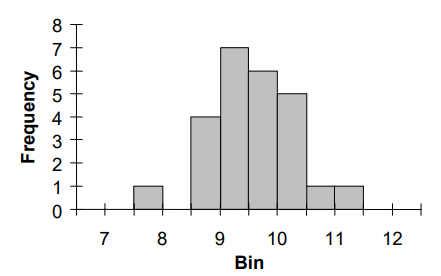
\includegraphics[width=0.5\linewidth]{fig_12_1}
		\label{fig:fig_12_1}
	\end{figure}
	\bigbreak


\section{ }
The data can be tabulated as
\bigbreak
	\begin{tabular}{ccc}
		\Xhline{1.5pt} i&y&$(y_{i}-\overline{y})^{2}$\\
		\hline1&28.65&0.390625\\
		2&28.65&0.390625\\
		3&27.65&0.140625\\
		4&29.25&1.500625\\
		5&26.55&2.175625\\
		6&29.65&2.640625\\
		7&28.45&0.180625\\
		8&27.65&0.140625\\
		9&26.65&1.890625\\
		10&27.85&0.030625\\
		11&28.65&0.390625\\
		12&28.65&0.390625\\
		13&27.65&0.140625\\
		14&27.05&0.950625\\
		15&28.45&0.180625\\
		16&27.65&0.140625\\
		17&27.35&0.455625\\
		18&28.25&0.050625\\
		19&31.65&13.14063\\
		20&28.55&0.275625\\
		21&28.35&0.105625\\
		22&28.85&0.680625\\
		23&26.35&2.805625\\
		24&27.65&0.140625\\
		25&26.85&1.380625\\
		26&26.75&1.625625\\
		27&27.75&0.075625\\
		28&\underline{27.25}&\underline{0.600625}\\
		$\bm\Sigma$&\bfseries784.7&\bfseries33.0125\\
		\Xhline{1.5pt}
	\end{tabular}
	\bigbreak
\begin{enumerate}[label=\bfseries(\alph*)]
	\bigbreak
\item$\overline{y}=\dfrac{784.7}{28}=28.025$
	\bigbreak
\item$s_{y}=\sqrt{\dfrac{33.0125}{28-1}}=1.105751$
	\bigbreak
\item$s_{y}^{2}=1.105751^{2}=1.222685$
	\bigbreak
\item$c.v.=\dfrac{1.105751}{28.025}\times100\%=3.95\%$
	\bigbreak
\item The data can be sorted and grouped.
	\bigbreak
	\begin{tabular}{ccc}
		\Xhline{1.5pt} lower&upper&$Frequency$\\
		\hline26&26.5&1\\
			26.5&27&4\\
			27&27.5&3\\
			27.5&28&7\\
			28&28.5&4\\
			28.5&29&6\\
			29&29.5&1\\
			29.5&30&1\\
			30&30.5&0\\
			30.5&31&0\\
			31&31.5&0\\
			31.5&32&1\\
		\Xhline{1.5pt}
	\end{tabular}
	\bigbreak
The histogram can then be constructed as
	\begin{figure}[H]
		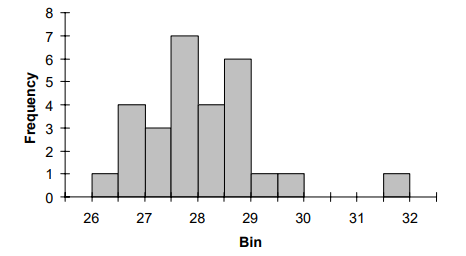
\includegraphics[width=0.5\linewidth]{fig_12_2}
		\label{fig:fig_12_2}
	\end{figure}
	\bigbreak
\item 68\% of the readings should fall between $\overline{y}-s_{y}$ and $\overline{y}+s_{y}$ . That is, between 28.025 –
1.10575096 = 26.919249 and 28.025 + 1.10575096 = 29.130751. Twenty values fall
between these bounds which is equal to 20/28 = 71.4\% of the values which is not that
far from 68\%. 
\end{enumerate}


\section{}
The sum of the squares of the residuals for this case can be written as
	\bigbreak
$\displaystyle S_r=\sum_{i=1}^{n} (y_{i}-a_{i}x_{i})^{2}$
	\bigbreak
The partial derivative of this function with respect to the single parameter a1 can be
determined as \bigbreak
$\displaystyle\dfrac{\delta S_r}{\delta a_1}=-2\sum\big[(y_{i}-a_{i}x_{i})x_{i}\big]$
	\bigbreak
Setting the derivative equal to zero and evaluating the summations gives \bigbreak 
$\displaystyle\sum y_{i}-a_{i}\sum x_{i}$
	\bigbreak
which can be solved for \bigbreak
$\displaystyle a_{i}=\dfrac{\sum y_{i}}{\sum x_{i}}$
	\bigbreak
\begin{blockquote}
So the slope that minimizes the sum of the squares of the residuals for a straight line with a
zero intercept is merely the ratio of the sum of the dependent variables (y) over the sum of
the independent variables (x). 
\end{blockquote}





\section{}
\begin{tabular}{ccccc}
		\Xhline{1.5pt} i&$x_{i}$&$y_{i}$&$x_{i}^{2}$&$x_{i}y_{i}$\\
		\hline1&0&9.8100&0&0\\
		2&20000&9.7487&4.0E+08&194974\\
		3&40000&9.6879&1.6E+09&387516\\
		4&60000&9.6278&3.6E+09&577668\\
		5&\underline80000&\underline9.5682&\underline6.4E+09&\underline765456\\
		$\bm\Sigma$&\bfseries200000&\bfseries48.4426&\bfseries1.2E+10&\bfseries1925614\\
		\Xhline{1.5pt}
\end{tabular}
	\bigbreak
$a_{1}=\dfrac{5(1,925,614)- 200,000(48.4426)}{5(1.2\times10^{-6})- 200,000^{2}}=-3.0225\times10^{-6}$
	\bigbreak
$a_{0}=\dfrac{48.4426}{5}-3.0225\times10^{-6}\dfrac{200,000}{5}=9.80492$
	\bigbreak
$g=6 9.80942-3.0225\times10^{-6}y$
	\bigbreak
The value at 55,000 m can therefore be computed as \bigbreak
$g=9.80942-3.0225\times10^{-6}(55,000)=9.6431825 6$
	\bigbreak

\section{}
Regresison gives
\bigbreak
\begin{align*}
\hspace{-2.8cm}p &= 8100.47 + 30.3164T & r^2 &= 0.999
\end{align*}
	\begin{figure}[H]
		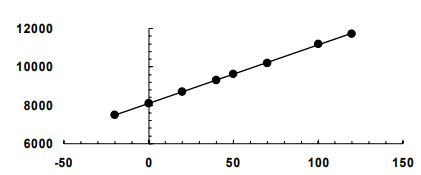
\includegraphics[width=0.5\linewidth]{fig_12_3}
		\label{fig:fig_12_3}
	\end{figure}
	\bigbreak
$R = \Big(\dfrac{p}{T}\Big)\dfrac{V}{n}$
	\bigbreak
$\dfrac{p}{T}=30.3164$
	\bigbreak
$n=\dfrac{1kg}{28g/mole}$
	\bigbreak
$R=30.3164\Big(\dfrac{10}{10^{3}/28}\Big)=8.487$
	\bigbreak
This is close to the standard value of 8.314 J/gmole.



\section{}
Linear regression gives
\bigbreak
	\begin{figure}[H]
		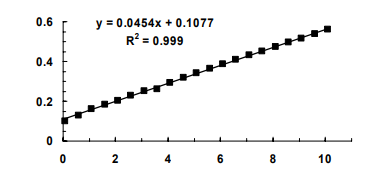
\includegraphics[width=0.5\linewidth]{fig_12_4}
		\label{fig:fig_12_4}
	\end{figure}
	\bigbreak
Forcing a zero intercept yields
	\begin{figure}[H]
		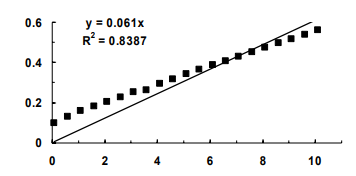
\includegraphics[width=0.5\linewidth]{fig_12_5}
		\label{fig:fig_12_5}
	\end{figure}
	\bigbreak
One alternative that would force a zero intercept is a power fit 
	\begin{figure}[H]
		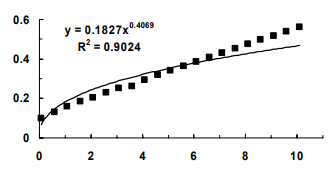
\includegraphics[width=0.5\linewidth]{fig_12_6}
		\label{fig:fig_12_6}
	\end{figure}
	\bigbreak
\begin{blockquote}
However, this seems to represent a poor compromise since it misses the linear trend in the
data. An alternative approach would to assume that the physically-unrealistic non-zero
intercept is an artifact of the measurement method. Therefore, if the linear slope is valid,
we might try y = 0.0454x.
\end{blockquote} 



\section{}
The function can be linearized by dividing it by x and taking the natural logarithm to yield
\bigbreak
$ln(y/x)=ln\alpha_{4}+\beta_4x$
	\bigbreak
\begin{blockquote}
Therefore, if the model holds, a plot of ln(y/x) versus x should yield a straight line with an
intercept of $ln\alpha_4$ and an intercept of $\beta_4$.
\end{blockquote}
	\bigbreak
	\begin{tabular}{ccc}
		\Xhline{1.5pt}x&y&ln(y/x)\\
		\hline0.1&0.75&2.014903\\
			0.2&1.25&1.832581\\
			0.4&1.45&1.287854\\
			0.6&1.25&0.733969\\
			0.9&0.85&-0.05716\\
			1.3&0.55&-0.8602\\
			1.5&0.35&-1.45529\\
			1.7&0.28&-1.80359\\
			1.8&0.18&-2.30259\\
		\Xhline{1.5pt}
	\end{tabular}
	\bigbreak
	\begin{figure}[H]
		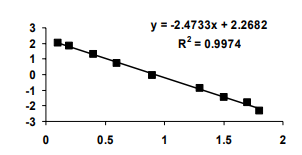
\includegraphics[width=0.5\linewidth]{fig_12_7}
		\label{fig:fig_12_7}
	\end{figure}
	\bigbreak
Therefore, $\beta_4=-2.4733$ and $\alpha_4=e^{2.2682}=9.661786$, and the fit is
	\bigbreak
	$y=9.661783xe^{-24733x}$
	\bigbreak
This equation can be plotted together with the data:
	\begin{figure}[H]
		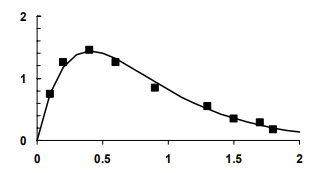
\includegraphics[width=0.5\linewidth]{fig_12_8}
		\label{fig:fig_12_8}
	\end{figure}



\section{}
The data can be transformed, plotted and fit with a straight line
\bigbreak
	\begin{tabular}{cccc}
		\Xhline{1.5pt}v, m/s&F,N&ln v&ln F\\
		\Xhline{1pt}10&25&2.302585&3.218876\\
			20&70&2.995732&4.248495\\
			30&380&3.401197&5.940171\\
			40&550&3.688879&6.309918\\
			50&610&3.912023&6.413459\\
			60&1220&4.094345&7.106606\\
			70&830&4.248495&6.721426\\
			80&1450&4.382027&7.279319\\
		\Xhline{1.5pt}
	\end{tabular}
	\bigbreak
	\begin{figure}[H]
		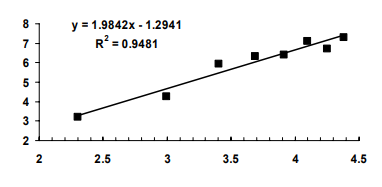
\includegraphics[width=0.5\linewidth]{fig_12_9}
		\label{fig:fig_12_9}
	\end{figure}
	\bigbreak
The least-squares fit is
	\bigbreak
$ln y = 1.9842ln x - 1.2941$
	\bigbreak
\begin{blockquote}
The exponent is 1.9842 and the leading coefficient is $e^{-1.2941} = 0.274137$. Therefore, the result is the same as when we used common or base-10 logarithms:
\end{blockquote}
	\bigbreak
$y = 0.274137x^{1.99842}$
	\bigbreak



\section{}
\begin{enumerate}[label=\bfseries(\alph*)]
\item The data can be plotted
\bigbreak
	\begin{figure}[H]
		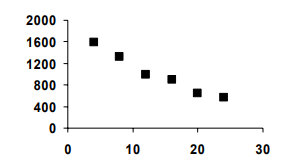
\includegraphics[width=0.5\linewidth]{fig_12_10}
		\label{fig:fig_12_10}
	\end{figure}
	\bigbreak
\begin{blockquote}
The plot indicates that the data is somewhat curvilinear. An exponential model (i.e., a semilog plot) is the best choice to linearize the data. This conclusion is based on%\item
\end{blockquote}
	\bigbreak
\begin{blockquote}
$\bullet$ A power model does not result in a linear plot\\
$\bullet$ Bacterial decay is known to follow an exponential model\\
$\bullet$ The exponential model by definition will not produce negative values.
\end{blockquote}
	\bigbreak
The exponential fit can be determined as
	\bigbreak
	\begin{tabular}{|c|c|r|}
		\hline t (hrs)&c (CFU/100 mL)&ln c\\ \hline
			4&1590&7.371489\\ \hline
			8&1320&7.185387\\ \hline
			12&1000&6.907755\\ \hline
			16&900&6.802395\\ \hline
			20&650&6.476972\\ \hline
			24&560&6.327937\\ \hline
	\end{tabular}
	\bigbreak
	\begin{figure}[H]
		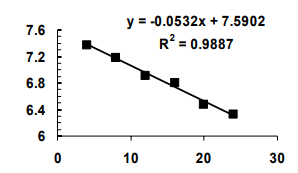
\includegraphics[width=0.5\linewidth]{fig_12_11}
		\label{fig:fig_12_11}
	\end{figure}
	\bigbreak
\begin{blockquote}
Therefore, the coefficient of the exponent $\beta_1$ is -0.0532 and the lead coefficient $\alpha_1$ is $e^{7.5902} = 1978.63$, and the fit is
\end{blockquote}
	\bigbreak
$c=1978.63e^{-0.0532t}$
	\bigbreak
\begin{blockquote}
Consequently the concentration at t = 0 is 1978.63 CFU/100 ml. Here is a plot of the fit along with the original data: 
\end{blockquote}
	\bigbreak
	\begin{figure}[H]
		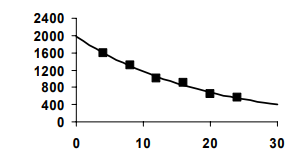
\includegraphics[width=0.5\linewidth]{fig_12_12}
		\label{fig:fig_12_12}
	\end{figure}
	\bigbreak
	\begin{tabular}{|c|c|r|}
		\hline t (hrs)&c (CFU/100 mL)&ln c\\ \hline
			4&1590&7.371489\\ \hline
			8&1320&7.185387\\ \hline
			12&1000&6.907755\\ \hline
			16&900&6.802395\\ \hline
			20&650&6.476972\\ \hline
			24&560&6.327937\\ \hline
	\end{tabular}
	\bigbreak
\item The time at which the concentration will reach 200 CFU/100 mL can be computed as
\end{enumerate}
	\bigbreak 
$200=1978.63e^{-0.0532t}$
	\bigbreak
$ln\Big(\dfrac{200}{1978.63}\Big)=-0.0532t$
	\bigbreak
$t=\dfrac{ln\Big(\dfrac{200}{1978.63}\Big)}{-0.0532}=43.08d$
	\bigbreak



\section{}
\begin{enumerate}[label=\bfseries(\alph*)]
\item The exponential fit can be determined with the base-10 logarithm as
\bigbreak
	\begin{tabular}{|c|c|r|}
		\hline t (hrs)&c (CFU/100 mL)&log c\\ \hline
			4&1590&3.201397\\ \hline
			8&1320&3.120574\\ \hline
			12&1000&3\\ \hline
			16&900&2.954243\\ \hline
			20&650&2.812913\\ \hline
			24&560&2.748188\\ \hline
	\end{tabular}
	\bigbreak
	\begin{figure}[H]
		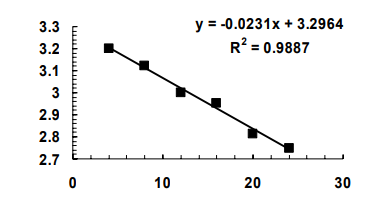
\includegraphics[width=0.5\linewidth]{fig_12_13}
		\label{fig:fig_12_13}
	\end{figure}
	\bigbreak
\begin{blockquote}
Therefore, the coefficient of the exponent $\beta_5$ is -0.231 and the lead coefficient $\alpha_5$ is $10^{3.2964} = 1978.63$, and the fit is 
\end{blockquote}
	\bigbreak
$c=1978.63(10)^{-0.0231t}$
	\bigbreak
Consequently the concentration at $t=0$ is 1978.63 CFU/100 mL can be computed as
\item The time at which the concentration will reach 200 CFU/100 mL can be computed as
\end{enumerate}
	\bigbreak 
$200=1978.63(10)^{-0.023lt}$
	\bigbreak
$ln\Big(\dfrac{200}{1978.63}\Big)=-0.023lt$
	\bigbreak
$t=\dfrac{ln\Big(\dfrac{200}{1978.63}\Big)}{-0.0231}=43.08d$
	\bigbreak
\begin{blockquote}
Thus, the results are identical to those obtained with the base-e model. The relationship between $\beta_1$ and $\beta_5$ can be developed as in 
\end{blockquote}
	\bigbreak
$e^{-a_1t}=10^{-a_5t}$
	\bigbreak
Take the natural log of this equation to yield
	\bigbreak
$-\alpha_1t=-\alpha_5tln10$
	\bigbreak
or
	\bigbreak
$\alpha_1=2.302585\alpha_5$
	\bigbreak



\section{}
The power fit can be determined as
\bigbreak
		\begin{tabular}{|c|c|c|c|}
		\hline W (kg)&$A(m^2)$&log W&log A\\ \hline
			70&2.1&1.845098&0.322219\\ \hline
			75&2.12&1.875061&0.326336\\ \hline
			77&2.15&1.886491&0.332438\\ \hline
			80&2.2&1.90309&0.342423\\ \hline
			82&2.22&1.913814&0.346353\\ \hline
			84&2.23&1.924279&0.348305\\ \hline
			87&2.26&1.939519&0.354108\\ \hline
			90&2.3&1.954243&0.361728\\ \hline
	\end{tabular}
	\bigbreak
	\begin{figure}[H]
		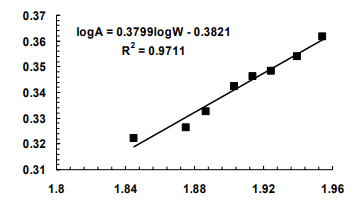
\includegraphics[width=0.5\linewidth]{fig_12_14}
		\label{fig:fig_12_14}
	\end{figure}
	\bigbreak
Therefore, the power is b = 0.3799 and the lead coefficient is $a=10^{-0.3821}=0.4149$, and the fit is
	\bigbreak
$A=0.4149W^{0.3799}$
	\bigbreak
Here is a plot of the fit along with the original data: 
	\bigbreak
	\begin{figure}[H]
		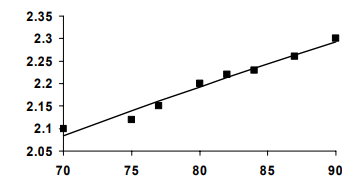
\includegraphics[width=0.5\linewidth]{fig_12_15}
		\label{fig:fig_12_15}
	\end{figure}
	\bigbreak
The value of the surface area for a 95-kg person can be estimated
	\bigbreak
$A=0.4149(95)^{0.3799}=2.34m^2$
	\bigbreak



\section{}
The power fit can be determined as
\bigbreak
		\begin{tabular}{|c|c|c|r|}
		\hline Mass&Metabolism&{}&{}\\
			(kg)&(kCal/day)&log Mass&log Met\\ \hline
			300&5600&2.477121&3.748188\\ \hline
			70&1700&1.845098&3.230449\\ \hline
			60&1100&1.778151&3.041393\\ \hline
			2&100&0.30103&2\\ \hline
			0.3&30&-0.52288&1.477121\\ \hline
	\end{tabular}
	\begin{figure}[H]
		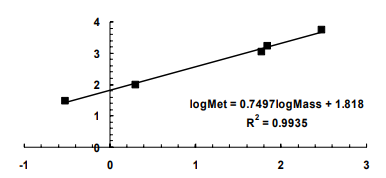
\includegraphics[width=0.5\linewidth]{fig_12_16}
		\label{fig:fig_12_16}
	\end{figure}
	\bigbreak
Therefore, the power is b = 0.7497 and the lead coefficient is $a = 10^{1.1818} = 65.768$, and the fit is
	\bigbreak
Metabolism = $65.768Mass^{0.7497}$
	\bigbreak
Here is a plot of the fit along with the original data: 
	\begin{figure}[H]
		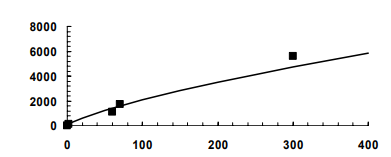
\includegraphics[width=0.5\linewidth]{fig_12_17}
		\label{fig:fig_12_17}
	\end{figure}
	\bigbreak



\section{}
Linear regression of the log transformed data yields
\bigbreak
\begin{align*}
\hspace{-2.8cm}log \epsilon &= -5.41 log B + 2.6363log\sigma & (r^2 &= 0.9997)
\end{align*}
	\begin{figure}[H]
		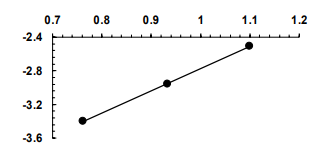
\includegraphics[width=0.5\linewidth]{fig_12_18}
		\label{fig:fig_12_18}
	\end{figure}
	\bigbreak
Therefore,
	\bigbreak
$B=10^{-5.41}=3.88975\times 10^{-6}$
	\bigbreak
$m=2.6363$
	\bigbreak
and the untransformed model is
	\bigbreak
$\epsilon=3.88975\times10^{-6}\sigma^{2.6363}$
	\bigbreak
A plot of the data and the model can be developed as
	\begin{figure}[H]
		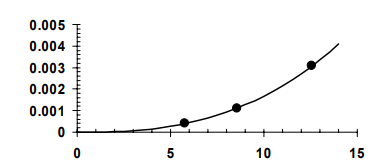
\includegraphics[width=0.5\linewidth]{fig_12_19}
		\label{fig:fig_12_19}
	\end{figure}
	\bigbreak



\section{}
Linear regression of the data yields
\bigbreak
\begin{align*}
\hspace{-2.8cm} \tau &= 2.779+0.685\gamma & (r^2 &= 0.977121)
\end{align*}
	\begin{figure}[H]
		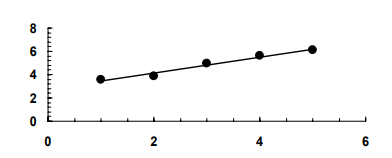
\includegraphics[width=0.5\linewidth]{fig_12_20}
		\label{fig:fig_12_20}
	\end{figure}
	\bigbreak
Therefore, $\mu=0.685$ and $\tau_y=2.779N/m^2$.
	\bigbreak


\section{}
The data can be transformed
\bigbreak
	\begin{tabular}{cccc}
		\Xhline{1.5pt}strain&stress&log(strain)&log(stress)\\
		\hline50&5.99&1.69897&0.777427\\
			70&7.45&1.845098&0.872156\\
			90&8.56&1.954243&0.932474\\
			110&9.09&2.041393&0.958564\\
			130&10.25&2.113943&1.010724\\
		\Xhline{1.5pt}
	\end{tabular}
	\bigbreak
Linear regression of the data yields
	\bigbreak

\begin{align*}
\hspace{-2.8cm} log\tau &= -0.13808+0.54298 log\gamma & (r^2 &= 0.989118)
\end{align*}
	\begin{figure}[H]
		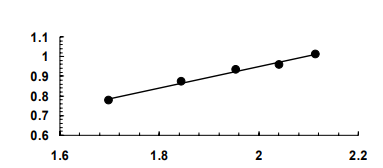
\includegraphics[width=0.5\linewidth]{fig_12_21}
		\label{fig:fig_12_21}
	\end{figure}
	\bigbreak
Therefore, $\mu=10^{-0.54298}=0.72765$ and $n=0.54298$. The power model is therefore, 
	\bigbreak
$\tau=0.72765\gamma^{0.54298}$
	\bigbreak
A plot of the power model along with the data can be created as
	\begin{figure}[H]
		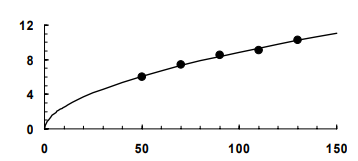
\includegraphics[width=0.5\linewidth]{fig_12_22}
		\label{fig:fig_12_22}
	\end{figure}
\end{document}